\documentclass{article}

\PassOptionsToPackage{numbers,sort&compress}{natbib}
\usepackage[dblblindworkshop,final]{neurips_2026}
\workshoptitle{Continual Learning in the Era of Foundation Models and Embodied Agents}

\usepackage[utf8]{inputenc}
\usepackage[T1]{fontenc}
\usepackage{amsmath,amssymb,amsfonts}
\usepackage{booktabs}
\usepackage{graphicx}
\usepackage{microtype}
\usepackage{xcolor}
\usepackage{hyperref}
\usepackage{url}

\hypersetup{
  hidelinks,
  pdfauthor={Szymon Hubert Duchowicz},
  pdftitle={Beyond Pairwise Task-Order Models: A Seed-Aware Spectral Audit of Continual-Learning Landscapes},
  pdfsubject={CL4FMAgents 2026 workshop paper},
  pdfkeywords={continual learning, task order, catastrophic forgetting, symmetric group, Fourier analysis}
}

\title{Beyond Pairwise Task-Order Models: A Seed-Aware Spectral Audit of Continual-Learning Landscapes}
\author{Szymon Hubert Duchowicz}
\date{}

\newcommand{\Sgroup}{S_K}
\newcommand{\Eplug}{E^{\mathrm{plug}}}
\newcommand{\Esig}{\widehat E^{\mathrm{sig}}}
\newcommand{\R}{\mathbb{R}}

\begin{document}

\maketitle

\begin{abstract}
Task order can change catastrophic forgetting, yet a good position-effect or transition model does not establish that pairwise structure is exactly sufficient. We introduce a seed-aware spectral audit for complete task-order experiments. The audit treats a scalar response over all task permutations as a function on the symmetric group, decomposes it by assignment degree, removes the diagonal seed-variation term when estimating reproducible signal, and jointly tests the entire higher-degree complement. In ten-seed MLP experiments containing every order, degree greater than two accounts for $16.1\%$ (approximate $95\%$ CI $[12.1\%,20.1\%]$) of estimated nonconstant signal at $K=5$ and $19.4\%$ ($[11.4\%,27.4\%]$) at $K=6$. Conditional on independent seed-level central symmetry, both whole-seed randomization tests reach the ten-seed resolution limit, $p=1/512$. A separate, explicitly post-selected analysis uses a complete $K=7$ landscape to illustrate how the audit localizes the residual within degree three. The result is a reusable distinction between low-degree approximation strength and exact structural sufficiency in continual-learning order effects.
\end{abstract}

\section{Introduction}

Continual learners acquire tasks sequentially and must retain prior competence while incorporating new tasks \citep{kirkpatrick2017overcoming,parisi2019continual}. Their final state can also depend on the curriculum: different orders change forgetting, generalization, and final performance \citep{bell2022ordering,lin2023theory}. For $K$ tasks, measuring one scalar response under every curriculum gives a complete task-order landscape
\begin{equation}
  F:\Sgroup\longrightarrow\R.
  \label{eq:landscape}
\end{equation}
This object contains more than a ranking. It can encode single task--position effects, paired assignments, and progressively higher-degree interactions among positions and tasks.

Position and transition scores are natural summaries of such landscapes. They are also useful scheduling models because they extrapolate from a small set of coefficients. Their predictive success, however, cannot establish that the underlying population landscape is exactly pairwise. Conversely, rejecting an exact pairwise model says nothing by itself about whether the residual is practically large. A useful audit should therefore answer two distinct questions: how much reproducible order signal is captured by degree at most two, and whether the population mean has exactly zero support outside that subspace.

We make that distinction precise using the representation theory of $S_K$. Noncommutative Fourier analysis decomposes the landscape into orthogonal isotypic blocks. Here $S_K$ acts on curriculum configurations rather than hidden representations, unlike group-equivariant architectures that constrain maps between feature spaces to respect group actions \citep{kondor2018equivariance}. The number of cells outside a partition's first row indexes an assignment-degree filtration, so the projection through degree two contains every position-effect and paired-assignment model, including adjacent-transition scores. Repeated training seeds add a second challenge. Training randomness materially affects machine-learning benchmarks \citep{bouthillier2021variance}, and squared coefficients of the seed mean algebraically mix population signal with this variation. We therefore estimate squared population-mean signal with cross-seed inner products and test the whole higher-degree coefficient vector using seed-level sign randomization.

The contributions are:
\begin{enumerate}
  \item an exact representation-theoretic identification of assignment degree and a joint test of degree-$\leq2$ support;
  \item seed-aware signal estimates that separate reproducible spectral energy from diagonal replicate noise, with uncertainty computed at the whole-landscape level;
  \item complete-order evidence at $K=5$ and $K=6$ showing that low-degree structure dominates but is not exactly sufficient, plus an explicitly exploratory $K=7$ allocation analysis; and
  \item a fail-closed reference implementation that validates complete permutation grids, representation identities, and provenance before publishing an audit.
\end{enumerate}

The claim is deliberately narrower than a universal law of curriculum learning. It concerns the spectral support of complete scalar forgetting landscapes for one MLP family. It does not identify causal mechanisms inside the network, nor does it say that a degree-two approximation is unusable. It directly tests a sharply defined model class for the measured landscapes.

\section{Related work}

\paragraph{Task ordering and continual learning.} Continual-learning research studies catastrophic forgetting, stability--plasticity, transfer, and mechanisms for retaining earlier competence \citep{kirkpatrick2017overcoming,parisi2019continual}. Complete five-task enumeration also predates this paper: \citet{singh2023learning} exhaustively evaluate five-class curricula while proposing an automated ranking method. For a different sequence-property objective, \citet{nguyen2019understanding} analyze $120$ permutations of a fixed five-task set. Other task-order work studies pairwise task relations \citep{bell2022ordering}, theoretical order dependence \citep{lin2023theory}, and optimization rules \citep{li2025optimal}. These approaches can reveal correlates or propose good curricula, but they do not jointly test whether all population-mean effects above assignment degree two vanish.

\paragraph{Permutation spectra and experimental design.} Orthogonal decomposition organizes classical factorial analysis \citep{speed1987anova}; finite-group Fourier analysis supplies the corresponding machinery for non-Abelian groups \citep{diaconis1988group}. Diaconis developed an ANOVA-like analysis of ranked data on $S_K$ \citep{diaconis1989ranked}. Later work studies transforms on permutations, fast low-frequency computation, spectral methods for experimental design, order-of-addition designs, and localized frames on the permutahedron \citep{huang2009fourier,plumb2015snfft,bailey2015spectraldesign,peng2019orderaddition,chen2021permutahedron}. The transform and exhaustive evaluation are therefore not our novelty. Our contribution is the replicated-response audit layer: assignment-degree estimands, seed-aware inference, a joint support test, dimension-aware drill-down, and provenance-bound outputs.

\paragraph{Inference.} The diagonal-free signal estimator is an order-two U-statistic \citep{hoeffding1948ustat}, related algebraically to inner-product estimators in high-dimensional mean testing \citep{chen2010twosample}. Delete-one uncertainty follows jackknife theory for U-statistics \citep{arvesen1969jackknife}. Whole-seed signs form a finite transformation group \citep{canay2017randomization,hemerik2018exact}; central symmetry is required for the finite-sample randomization guarantee. Holm adjustment controls fixed component families \citep{holm1979multiple}, but it does not by itself account for an earlier data-dependent choice of which component family to report \citep{berk2013postselection}.

\section{Seed-aware spectral audit}

\subsection{Input and Fourier decomposition}

The audit accepts $M$ scalar landscapes $F_m:\Sgroup\to\R$ on a common complete permutation grid. Before analysis it checks $K$, exact $K!$ coverage, duplicate or inconsistent labels, finite responses, seed identity, array layout, and source hashes. One landscape supports a descriptive decomposition; repeated independent seeds enable population-signal estimation and inference.

Let $G=|S_K|=K!$, and let $\lambda\vdash K$ index an irreducible orthogonal representation $\rho_\lambda$ of dimension $d_\lambda$. For a complete landscape $F$, define the unnormalized transform and normalized block energy
\begin{equation}
  \widehat F_\lambda=\sum_{g\in S_K}F(g)\rho_\lambda(g),\qquad
  E_\lambda(F)=\frac{d_\lambda}{G^2}\lVert\widehat F_\lambda\rVert_F^2,\qquad
  \frac{\lVert F\rVert_2^2}{G}=\sum_{\lambda\vdash K}E_\lambda(F).
  \label{eq:spectrum}
\end{equation}
The last equality is Parseval's identity under this normalization \citep{diaconis1988group}. The trivial block $(K)$ is the grand mean; order-effect fractions exclude it. The implementation constructs Young's orthogonal matrices directly from tableau axial distances; see Sagan's adjacent-transposition seminormal construction \citep[Ex.~2.12.11]{sagan2001symmetric}.

\subsection{Assignment degree}

Write $x_{pi}(\pi)=\mathbf 1\{\pi(p)=i\}$. Consistent assignment monomials through degree $k$ span
\begin{equation}
  \mathcal V_{\leq k}:=\operatorname{span}\!\left\{\prod_{r=1}^{t}x_{p_ri_r}:0\leq t\leq k\right\}
  =\bigoplus_{K-\lambda_1\leq k}\mathcal I_\lambda,
  \qquad \operatorname{ord}(\lambda):=K-\lambda_1,
  \label{eq:degree}
\end{equation}
where $\mathcal I_\lambda$ is the full regular isotypic component. Appendix~\ref{app:proof} gives the proof. Degree one contains translated task--position effects; degree two contains every translated paired assignment. Projection onto $\mathcal V_{\leq k}$ is therefore the best complete-grid least-squares reconstruction at assignment degree $k$.

An adjacent-transition score is explicitly degree two:
\begin{equation}
  \sum_{p=1}^{K-1}a_{\pi(p),\pi(p+1)}
  =\sum_{p=1}^{K-1}\sum_{i\ne j}a_{ij}x_{pi}x_{p+1,j}.
  \label{eq:transition}
\end{equation}
Thus rejecting degree-$\leq2$ support rules out exact sufficiency of an entire class containing position and transition models, rather than only one fitted parameterization. It does not show that every individual higher-degree block is nonzero.

\subsection{Population signal and the joint null}

For seed $m$, let $H_{m,\lambda}=\sum_gF_m(g)\rho_\lambda(g)$. Squaring the coefficient of the seed mean gives a useful descriptive plug-in energy but includes a diagonal seed-variation term. We instead estimate squared population-mean signal with
\begin{equation}
  \Esig_\lambda=
  \frac{d_\lambda}{G^2M(M-1)}
  \sum_{i\ne j}\langle H_{i,\lambda},H_{j,\lambda}\rangle_F.
  \label{eq:ustat}
\end{equation}
Under independent identically distributed seeds and finite second moments, cross-seed inner products make Eq.~\eqref{eq:ustat} unbiased for $d_\lambda\lVert\mathbb EH_{m,\lambda}\rVert_F^2/G^2$. Estimates remain untruncated, so weak signal can yield a negative estimate. Fractions recompute the numerator and nontrivial denominator together in every delete-one replicate; intervals are marked unavailable when a required denominator is nonpositive.

To test exact degree-$\leq2$ support, concatenate all scaled higher-degree blocks,
\begin{equation}
  Z_m^{>2}=\bigoplus_{\operatorname{ord}(\lambda)>2}
  \frac{\sqrt{d_\lambda}}{G}\operatorname{vec}(H_{m,\lambda}),
  \qquad H_0:\mathbb EZ_m^{>2}=0.
  \label{eq:jointnull}
\end{equation}
The statistic is the squared norm of the signed seed mean. Flipping each seed's whole vector preserves dependence among partitions and coordinates. At $M=10$, fixing one sign removes the duplicate global-sign orbit and leaves $2^{M-1}=512$ classes; upper-tail ties count against rejection. The resulting $p$-value is finite-sample valid under independent seed-level central symmetry. Independent seeding and mean zero do not imply that assumption. Approximate $95\%$ intervals use delete-one-seed jackknife standard errors with a $t_{M-1}$ reference.

\subsection{Within-degree allocation}

A regular-representation block $\lambda$ has $d_\lambda^2$ coordinates. Within a degree family $\mathcal L_o$, a dimension-only allocation baseline is therefore
\begin{equation}
  q_\lambda=\frac{d_\lambda^2}{\sum_{\mu\in\mathcal L_o}d_\mu^2},
  \qquad C_h=\Esig_h-q_h\Esig_o.
  \label{eq:allocation}
\end{equation}
The contrast asks whether a chosen block receives more population signal than its coordinate share. This geometric baseline is not a mechanistic null. A target selected after inspecting the same spectra remains exploratory even when the reported family receives multiplicity adjustment.

\section{Complete-order forgetting experiments}

For curriculum $\pi$, let $a_\tau^{\mathrm{post}}(\pi)$ be task $\tau$'s accuracy immediately after its block and $a_\tau^{\mathrm{final}}(\pi)$ its accuracy after the sequence. We audit total forgetting
\begin{equation}
  F_{\mathrm{seq}}(\pi)=\sum_{\tau=1}^K\left(a_\tau^{\mathrm{post}}(\pi)-a_\tau^{\mathrm{final}}(\pi)\right).
  \label{eq:forgetting}
\end{equation}
Each experiment uses a two-hidden-layer width-$64$ multi-head MLP with a shared ReLU trunk, SGD with momentum, and ten seeds controlling initialization and minibatch order. The $K=5$ battery contains five disjoint binary MNIST tasks \citep{lecun1998gradient} and all $120$ orders. The $K=6$ battery contains three MNIST and three Fashion-MNIST \citep{xiao2017fashion} binary tasks and all $720$ orders. These two audits support the primary support claim.

We also retain a complete $K=7$ landscape with $5{,}040$ orders and ten seed responses. It appends MNIST $\{6,7\}$ to the mixed six-task battery. Its current array passes permutation, layout, Parseval, and dimension checks, but its metadata schema was reconstructed retrospectively without retraining, and its seed labels differ from the $K=5,6$ experiments. We therefore use $K=7$ only in the post-selected allocation illustration. Comparisons across $K$ are not scaling laws because battery composition changes with $K$.

\section{Results}

\subsection{Degree two dominates but is not exact}

\begin{figure*}[t]
  \centering
  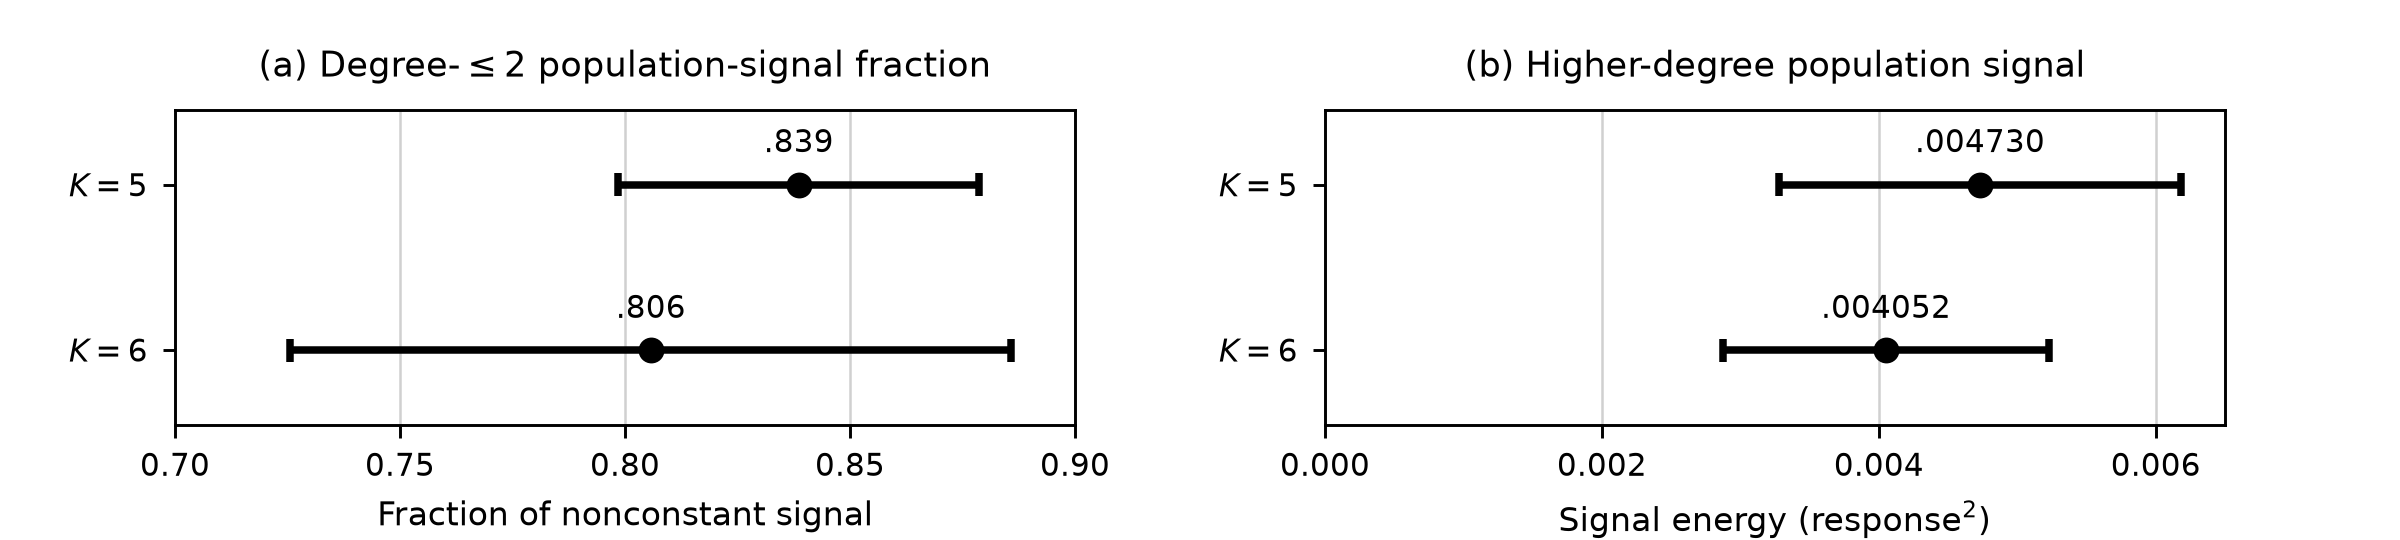
\includegraphics[width=.90\textwidth]{figures/figure1_population_signal.png}
  \caption{Population-signal summary for the two primary complete-order audits. Points are estimates and bars are approximate $95\%$ delete-one-seed jackknife-$t$ intervals. The right panel reports response-squared units. Both whole-seed sign-randomization tests give $p=1/512=.001953$.}
  \label{fig:signal}
\end{figure*}

\begin{table}[t]
  \caption{Primary audit of degree-$\leq2$ sufficiency. Fractions exclude the trivial mean block.}
  \label{tab:primary}
  \centering
  \small
  \begin{tabular}{@{}rcccc@{}}
    \toprule
    $K$ & plug-in fraction $\leq2$ & signal fraction $\leq2$ (95\% CI) & $\Esig_{>2}$ (95\% CI) & $p$ \\
    \midrule
    5 & .836 & .839 [.799,.879] & .004730 [.003279,.006182] & .001953 \\
    6 & .781 & .806 [.726,.886] & .004052 [.002872,.005232] & .001953 \\
    \bottomrule
  \end{tabular}
\end{table}

Degree at most two contains about four fifths of reproducible nonconstant signal in both batteries. The complement nevertheless accounts for $16.1\%$ at $K=5$ and $19.4\%$ at $K=6$, with intervals shown in Fig.~\ref{fig:signal}. In RMS units, the orthogonal higher-degree component is approximately $40\%$ and $44\%$ as large as the full nonconstant population signal, respectively. The residual is therefore neither dominant nor negligible.

Each $p$-value is the ten-seed enumeration floor. More precisely, the observed squared norm is uniquely largest among all $512$ whole-seed sign classes modulo global sign. This is a resolution-limited rank statement, not an effect-size measure; the signal fractions and intervals carry the magnitude information. Conditional on the stated central-symmetry assumption, we reject exact degree-$\leq2$ support in each primary experiment.

For curriculum modeling, the interpretation is direct. Every position-effect and transition model in Eq.~\eqref{eq:transition} lies in $\mathcal V_{\leq2}$, so no member of that entire class can exactly equal these population-mean landscapes. The same models may still be useful approximations, and the audit does not choose an application-specific tolerance. It separates the approximation decision from the structural conclusion.

\subsection{Where the degree-three remainder lies}

Within degree three, the visually prominent block follows the near-hook pattern $h_K=(K-3,2,1)$. Because this pattern was chosen after inspecting the spectra, Table~\ref{tab:allocation} is a post-selected diagnostic rather than confirmatory discovery. It compares signal share only with the squared-dimension coordinate baseline from Eq.~\eqref{eq:allocation}.

\begin{table}[t]
  \caption{Exploratory near-hook allocation within degree three. Two-sided values use Holm adjustment across the three displayed batteries, conditional on the selected pattern.}
  \label{tab:allocation}
  \centering
  \small
  \begin{tabular}{@{}ccccc@{}}
    \toprule
    $K$ & $h_K$ & coordinate baseline & signal share (95\% CI) & $p_{\mathrm{Holm}}$ \\
    \midrule
    5 & $(2,2,1)$ & .6098 & .9536 [.8705,1.0000] & $1.42\!\times\!10^{-4}$ \\
    6 & $(3,2,1)$ & .6719 & .8004 [.6841,.9211] & .0351 \\
    7 & $(4,2,1)$ & .6727 & .8158 [.7663,.8836] & $1.42\!\times\!10^{-4}$ \\
    \bottomrule
  \end{tabular}
\end{table}

The near-hook receives more estimated degree-three signal than its coordinate share in all three batteries. This is stronger than observing that it is the largest block, but weaker than a selection-free discovery claim. The $K=6$ contrast is the least stable, and adjustment across $K$ does not correct the earlier choice of the partition pattern. At $K=5$ and $K=6$, the mean coefficient matrices are also descriptively concentrated: their leading singular directions contain $78\%$ and $66\%$ of block energy, with effective ranks $1.56$ (seed-resampling interval $[1.40,1.81]$) and $2.17$ ($[2.01,3.30]$). These summaries localize structure; they do not identify parameter counts or a causal neural mechanism.

\begin{figure}[t]
  \centering
  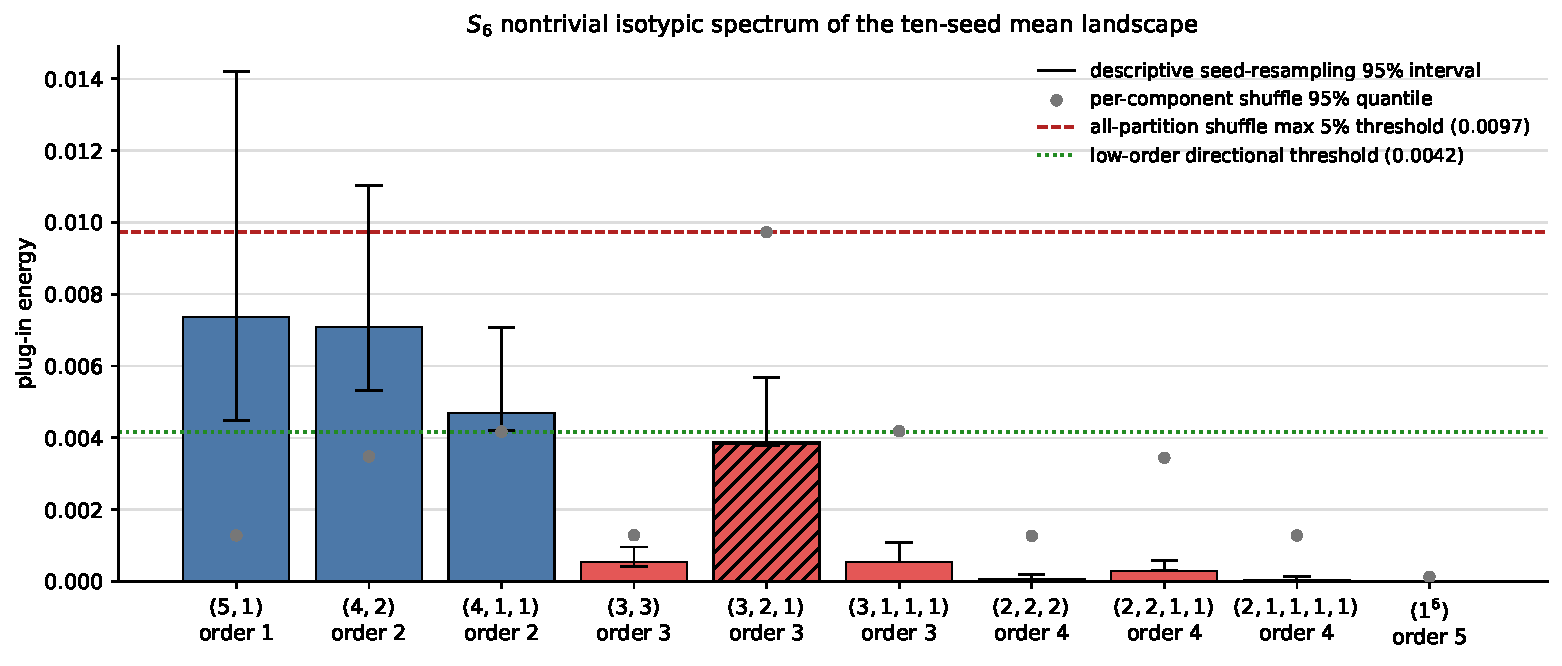
\includegraphics[width=.92\linewidth]{figures/figure_2_spectrum_k6.pdf}
  \caption{Descriptive $K=6$ plug-in partition spectrum. Orders through two capture $78.1\%$ of observed nonconstant variation; adding degree three raises the complete-grid reconstruction ceiling to $98.3\%$. The hatched bar is the post-selected near-hook. Shuffle references diagnose allocation under label exchangeability and are not the seed-level zero test.}
  \label{fig:k6spectrum}
\end{figure}

Figure~\ref{fig:k6spectrum} illustrates why the audit has layers. The descriptive spectrum shows dominance, the cross-seed estimator measures reproducible allocation, the omnibus test addresses exact support, and the within-degree contrast localizes a selected remainder. None of these conclusions follows automatically from another.

\section{Reference implementation and scaling}

The command-line implementation consumes explicit permutation, response, seed, and layout fields. It fails closed on incomplete or duplicated grids, nonfinite values, inconsistent layouts, and repeated seed identifiers. Before publishing a result bundle it verifies Parseval and representation dimensions, writes tables atomically, and records source, configuration, implementation, diagnostic, and output hashes in a manifest. A single-landscape mode returns exact descriptive projections while withholding population intervals and sign tests.

The exact transform scales with $K!$. On synthetic deterministic ten-seed landscapes, a complete in-memory audit takes $0.017$, $0.029$, $0.126$, and $1.406$ seconds for $K=4,5,6,7$, with median peak resident memory $36.0$, $36.4$, $40.9$, and $154.9$ MiB on the recorded Windows 11 benchmark system. These are audit costs, not training costs. Training every curriculum remains the bottleneck; sampled curricula require a different estimator that accounts jointly for incomplete group coverage and seed variation.

\section{Limitations and discussion}

The primary evidence uses only ten seeds. Independent random seeding does not imply joint central symmetry of the high-dimensional seed vectors, and ten vectors cannot validate that assumption reliably. The randomization conclusions are therefore conditional. The cross-seed signal estimator itself does not require symmetry, while its jackknife-$t_9$ intervals are approximate rather than finite-sample coverage guarantees. The $1/512$ floor limits inferential resolution.

The empirical scope is also narrow. The primary batteries differ in task composition, use one MLP family, and measure one scalar response. Their numerical differences are not evidence of a scaling law or architectural generality. The $K=7$ allocation result has an additional retrospective-provenance qualification and is post-selected. A confirmatory study should fix the target partition before inspection or separate selection from evaluation.

Finally, spectral blocks describe structure in curriculum space, not causal mechanisms inside a network. Many nonlinear training processes can induce a low-degree scalar response after aggregation over tasks and seeds. The observed combination is consequently plausible but informative: roughly four fifths of reproducible signal lies in position and paired-assignment structure, while a coherent higher-degree remainder rules out exact pairwise sufficiency. For continual-learning practice, the tool supplies a falsification test and effect decomposition, not a universal scheduler.

\section{Conclusion}

A complete task-order experiment is a repeated function on $S_K$. The proposed audit converts it into two outputs that curriculum studies often conflate: approximation strength and exact structural support. In the two primary forgetting landscapes, degree at most two captures most reproducible signal but is not exactly sufficient. An exploratory drill-down shows how a selected part of the remainder can be localized without elevating it into a universal mechanism. The durable contribution is a seed-aware, provenance-validated method for determining what order-effect models can and cannot represent exactly.

\section*{Acknowledgments}
I thank Adam Wróbel for his mentorship, which helped me develop my research skills, and Prof. Bartosz Zieli{\fontencoding{OT1}\selectfont\'{n}}ski for making this mentorship possible.

\clearpage
\bibliographystyle{plainnat}
\bibliography{references}

\clearpage
\appendix

\section{Assignment-degree proof}
\label{app:proof}

After repeated factors are deleted, every nonzero degree-$t$ monomial in Eq.~\eqref{eq:degree} is an indicator of an ordered $t$-coset. Its left and right translates are matrix coefficients of the permutation module
\begin{equation}
  M^{(K-t,1^t)}=\operatorname{Ind}_{S_{K-t}}^{S_K}\mathbf1.
\end{equation}
Young's rule gives exactly the irreducible constituents $S^\lambda$ with $\lambda\unrhd(K-t,1^t)$, equivalently $\lambda_1\geq K-t$. Their matrix coefficients span the corresponding complete regular isotypic components. Taking the span over $t\leq k$ proves Eq.~\eqref{eq:degree}; orthogonal subtraction isolates exact degree $k$. This is the ordered-coset span theorem of \citet[Theorem~7]{ellis2011intersecting}, stated directly in low-degree/largest-first-row language by \citet[Theorem~1]{ellis2017lowdegree}. Equivalent polynomial and Fourier-support notions are discussed by \citet{dafni2021complexity}.

The statement concerns the span over all task and position choices. It does not say that a degree-$k$ component depends on one fixed $k$-tuple. Degree zero is the mean, degree one is $(K-1,1)$, and degree two comprises $(K-2,2)$ and $(K-2,1,1)$.

\section{Inferential details}

For any fixed partition family $\mathcal A$, summing Eq.~\eqref{eq:ustat} remains unbiased for the corresponding population squared norm. Delete-one replicates recompute all U-statistics from the remaining nine seeds. Fractions and allocation shares recompute numerator and denominator together, and an interval is omitted when the full-sample or a required leave-one-out denominator is nonpositive.

The sign statistic is the squared norm of the signed seed mean after concatenation. Whole-seed signs preserve covariance among coordinates and partitions; coordinate-wise signs do not. Fixing one sign removes the duplicate global-sign orbit. Upper-tail ties are included. A component family, when requested, uses Holm correction; the degree-wide omnibus is one joint hypothesis and needs no component-wise adjustment.

\section{Additional numerical results}

\subsection{Full $K=5$ descriptive spectrum}

\begin{table}[h]
  \caption{$K=5$ plug-in partition spectrum. Fractions are shares of observed nonconstant variation.}
  \centering
  \small
  \begin{tabular}{@{}crrr@{}}
    \toprule
    $\lambda$ & $d_\lambda$ & degree & plug-in energy (share) \\
    \midrule
    $(4,1)$ & 4 & 1 & .0046 (.153) \\
    $(3,2)$ & 5 & 2 & .0167 (.549) \\
    $(3,1,1)$ & 6 & 2 & .0041 (.135) \\
    $(2,2,1)$ & 5 & 3 & .0046 (.153) \\
    $(2,1,1,1)$ & 4 & 3 & .0003 (.010) \\
    $(1^5)$ & 1 & 4 & $<.0001$ (.0003) \\
    \bottomrule
  \end{tabular}
\end{table}

\subsection{$K=6$ complete-grid projection ceilings}

\begin{table}[h]
  \caption{Descriptive projections of the observed $K=6$ ten-seed mean. These are complete-grid reconstruction ceilings, not held-out performance.}
  \centering
  \small
  \begin{tabular}{@{}rrrr@{}}
    \toprule
    maximum degree & subspace dimension & $R^2$ ceiling & increment \\
    \midrule
    0 & 1 & .000000 & .000000 \\
    1 & 26 & .300413 & .300413 \\
    2 & 207 & .781254 & .480841 \\
    3 & 588 & .983105 & .201850 \\
    4 & 719 & .999993 & .016888 \\
    5 & 720 & 1.000000 & .000007 \\
    \bottomrule
  \end{tabular}
\end{table}

\section{Reproducibility and artifact scope}

The numerical audit environment records Python 3.14.6 and NumPy 2.4.4. The supporting artifact is available at \href{https://anonymous.4open.science/r/taskorder-spectral-audit-C3D1}{browse repository or download ZIP}. It contains the manuscript, bibliography, unmodified NeurIPS style, figure assets, validated claim CSVs, exact build instructions, the BSD-3-Clause package source, focused tests, benchmark CSVs, and scalar landscape arrays. It excludes raw MNIST or Fashion-MNIST archives, training logs, historical drafts, cache files, and machine-specific paths. A SHA-256 manifest binds every packaged member, while separate claim and package verifiers check the displayed values, provenance chains, and release surface.

Training all $K!$ curricula is not reproduced by the audit package. Existing training records describe tasks, architecture, optimizer, seeds, shuffle behavior, and the forgetting response, but do not establish bitwise reproducibility across numerical-library builds or GPU kernels. The $K=7$ metadata limitation described in the main text is retained in the repository documentation.

\end{document}
